\chapter{Computational Methods} \label{chap:comp_met}

\section{Software: OpenFOAM and LIGGGHTS}
An implementation of the method derived in the Chapter \ref{chap:lit_rev} based on OpenFOAM\textsuperscript{\textregistered} \cite{jasak2007openfoam} open-source programming library which includes Finite Volume Method (FVM) solvers using its tools and data structures. A solver is made up of two main parts: a main structure and a number of extensions or tools. The main structure solves the governing equations, while the other part could be used for a specific tasks like: mesh decomposition, refinement or methods for solution of final system of equation. The solver is 3D and could be run in parallel.
% i mean this will be methods for matrix inversion etc

Another part of the method is solving and coupling with OpenFoam solid movement part using Discrete Element Method (DEM) with LIGGGHTS\textsuperscript{\textregistered} package which is coupled with OpenFOAM through CFDEMcoupling \cite{kloss2011liggghts}. LIGGGHTS® is based on LAMMPS \cite{LAMMPS} a classical molecular dynamics simulator based on the time integration algorithm using Verlet symplectic integrator \cite{verlet}. The code is written in C++ and makes extensive use of templates. This design approach enhances the framework's flexibility and extensibility, enabling both users and developers to introduce custom algorithms, solvers, and utilities without modifying the core architecture. One other benefit of using LIGGGHTS®, that it supports large scale parallelism. Distributed-memory parallelism via MPI\cite{MPI} with different ways of spatial decomposition. This all give opportunity to run the whole simulation in parallel on an HPC cluster and significantly improve compuatational time .

\section{Implementation: cfdemSolverInterFlowIB}
For this work we implemented and tested two solvers \verb|cfdemSolverInterFlowIB| and \verb|cfddemSolverMultisphereIB|. The difference between them is in the approaches which was used for free surface reconstruction. First uses isoAdector alogorythm and the other one based on MULES \cite{MULES} algorithm, which was discussed in the first chapter.

When introducing particles into a fluid field, their presence is accounted for by incorporating an external body force term in the momentum equation. This approach ensures an appropriate representation of the impact of the particles on the fluid dynamics. Once this term is added, the momentum equation is discretized. However, it's crucial also to consider the reciprocal effect, specifically the hydrodynamic forces exerted on the particles by the fluid. This interaction is a result of the coupled nature of the particle-fluid environment. The influence of the fluid flow on the particles is determined by two factors: the hydrodynamic drag force and the viscous stress from the fluid. The hydrodynamic drag arises due to the pressure across the particle, while the viscous stress is attributed to the fluid's viscosity. These forces play a significant role in determining the particle's motion and behavior within the fluid field.

The schematic description implementation of  \verb|cfdemSolverInterFlowIB| is shown on the Figure \ref{fig:cfddemSolver} below. 
\begin{figure}[!ht]
    \centering
    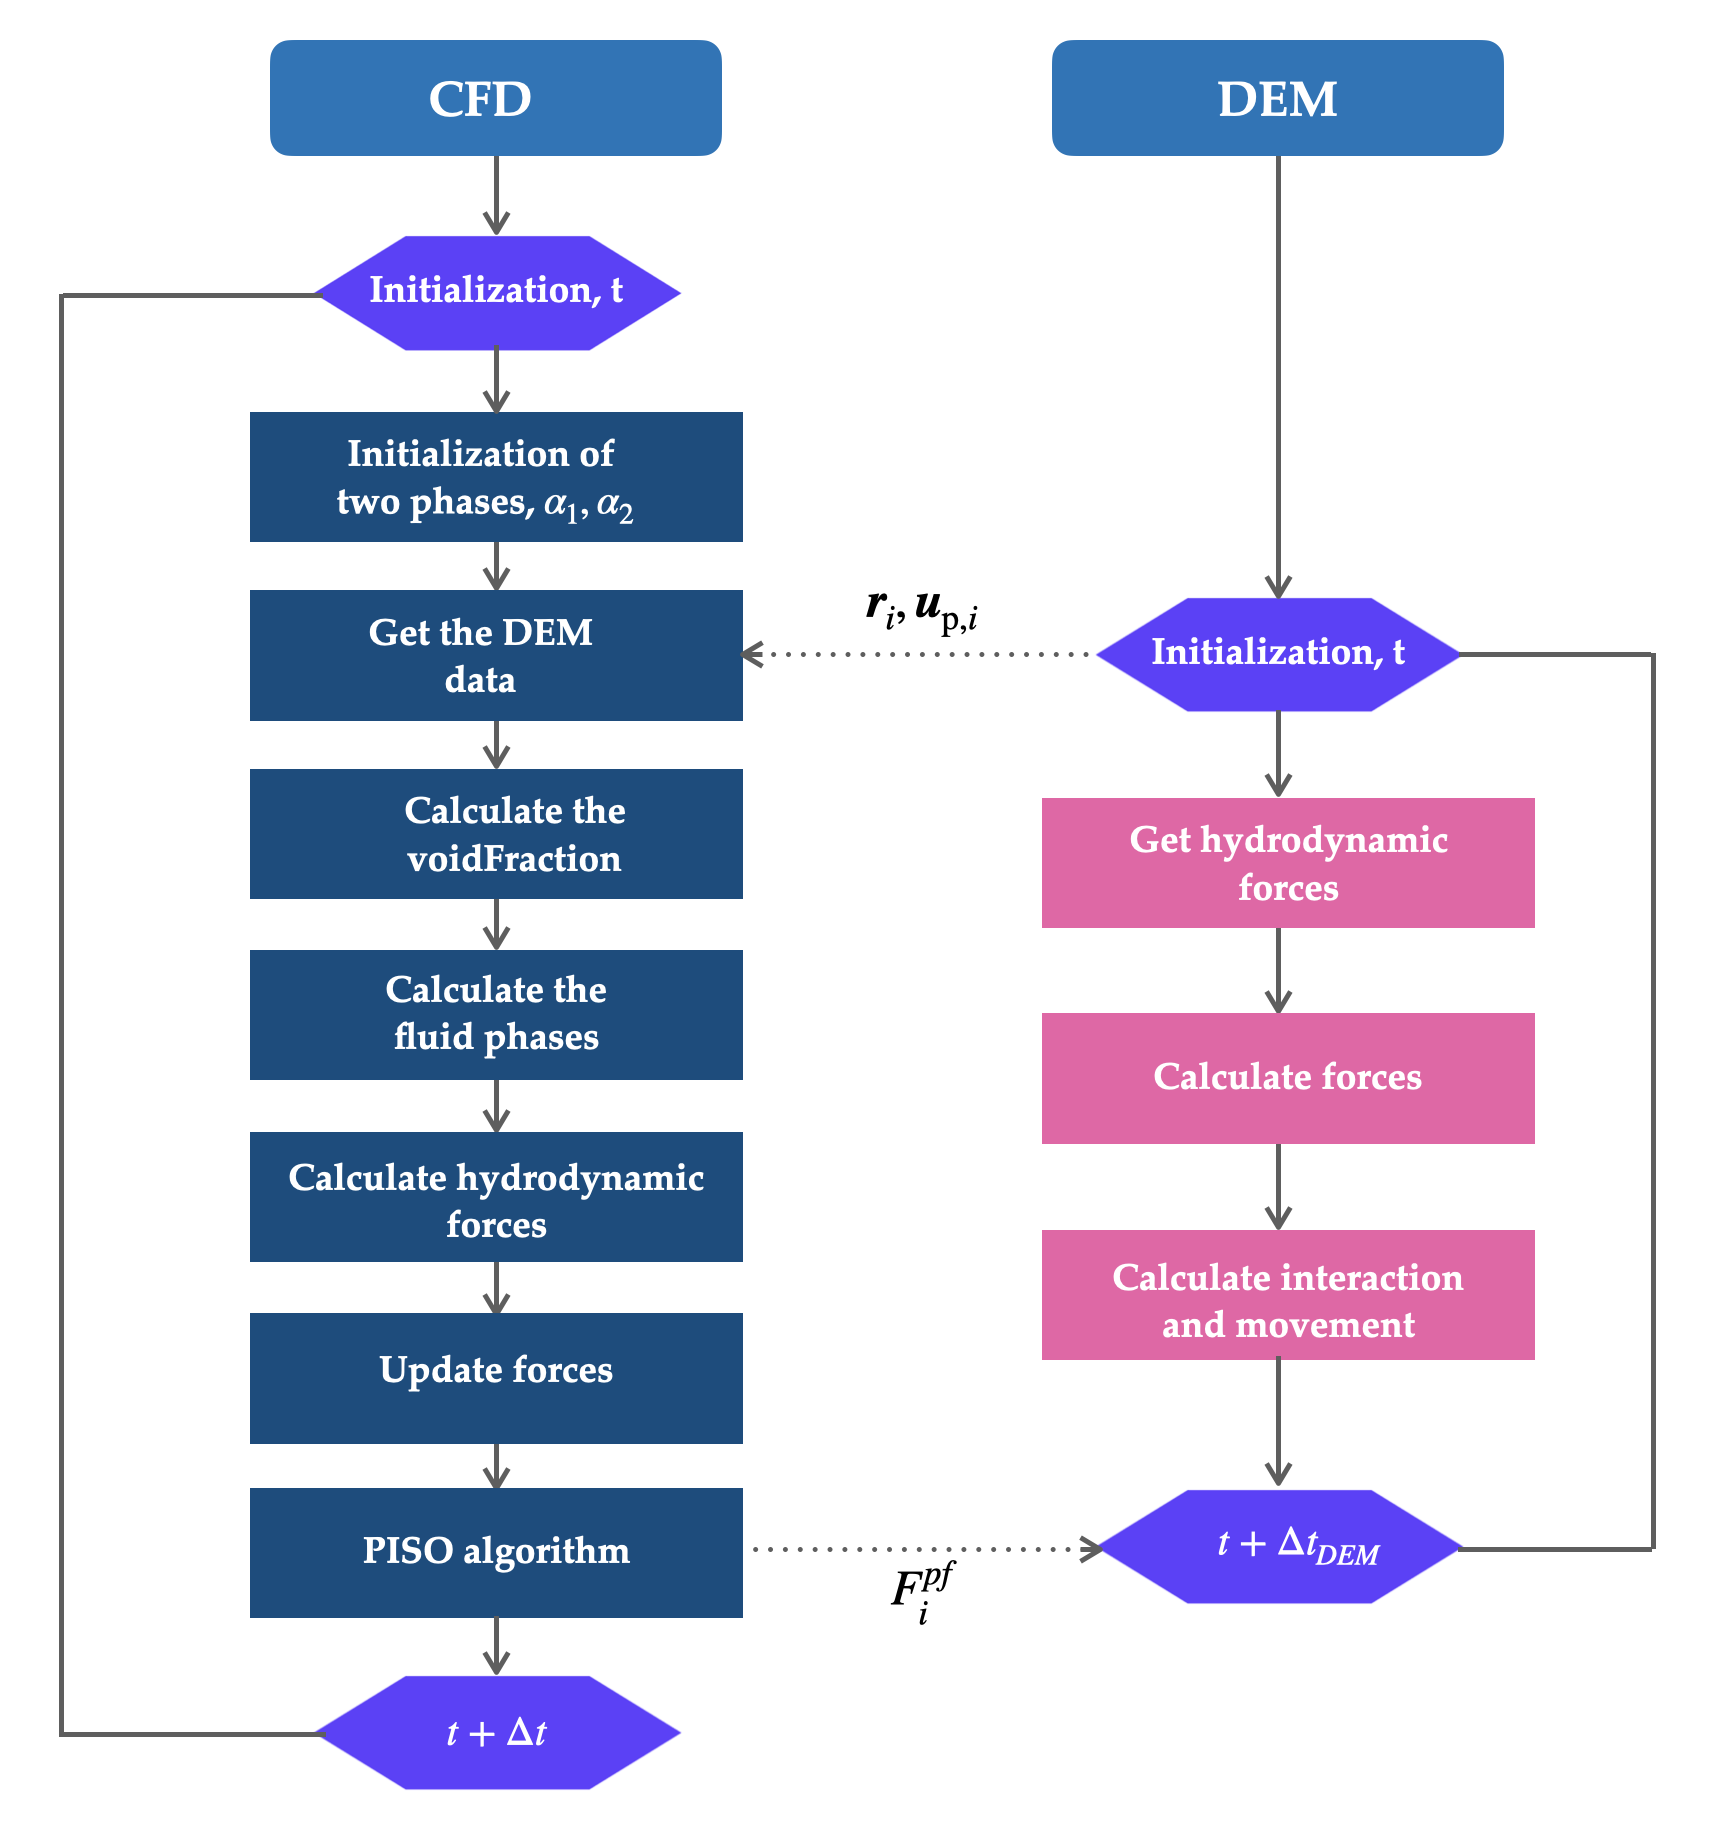
\includegraphics[width=17cm]{Images/chap3/CFD-DEM_scheme.png}
    \caption{Schematic description of resolved CFD-DEM solver.}
    \label{fig:cfddemSolver}
\end{figure}
\begin{itemize}
    \item First we need to initialize and decompose CFD mesh, after this  we initialize two phases, marking each cell of CFD in the range $[0,1]$ based on IsoAdvector method \cite{roenby2019isoadvector}.
    \item  After initialization of CFD we initialize DEM part by determining positions, velocity and radius of each particle in the domain.
    \item Then we sending data to CFD mesh identifying cells occupied with solid bodies and save this cells as a \textit{voidFraction} field. 
    \item Then we starting PISO loop. First, solve momentum equation based on velocity fluid field from previous step with two phases and \textit{voidFraction} field also from the previous step or based on initial conditions.
    \item In the PISO loop we also calculating the hydrodynamic forces acting on the particles with \textit{forceModel} and then the data is send to the DEM part
    \item The last step is pressure and velocity correction, finishing PISO loop and moving on to the next step.
\end{itemize}

The step of force calculation is the most important part of the simulation. For this goal we need to calculate interaction between the fluid and the particle which is calculated in the CFD part of the solver and called \textit{forceModel}. It responsible for computing the fluid-particle interaction force, taking into account various physical phenomena, and relays this information to the DEM module to update particle data. In dealing with different physical interactions, it is crucial to incorporate the corresponding physics into the \textit{forceModel} implementation. These models encompass a range of interactions, including viscous and pressure drag forces exerted on the particle by the flow, lift forces arising from density differences between the particle and the fluid, among others. 

\begin{figure}[!ht]
    \centering
    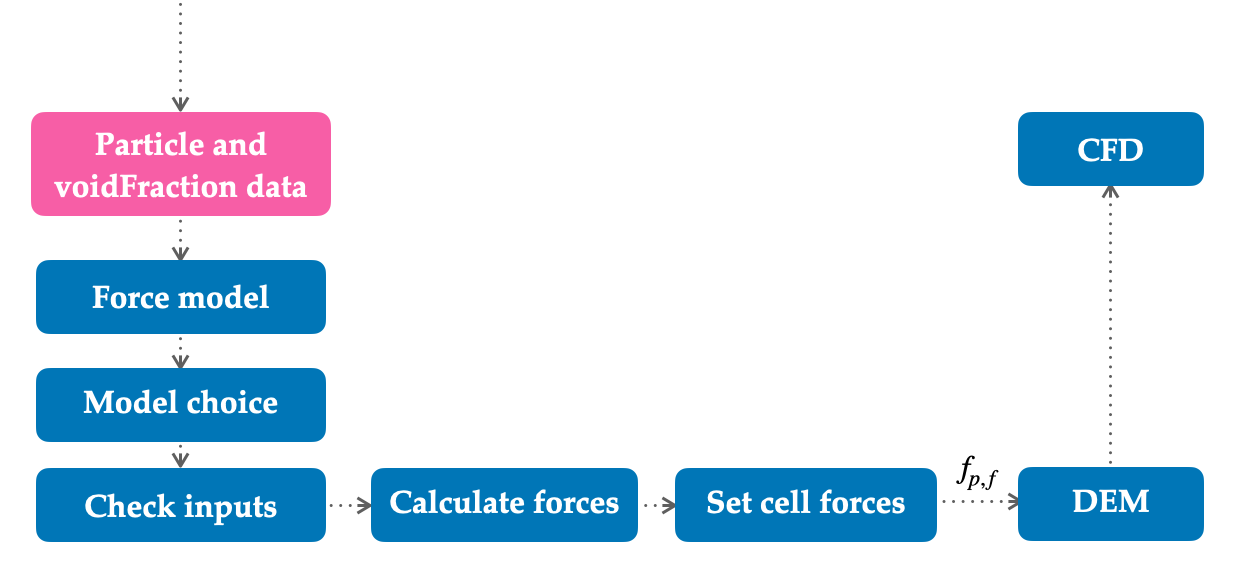
\includegraphics[width=15cm]{GWU_Thesis_Sarmakeeva/Images/chap3/force_model.png}
    \caption{Schematic description how force model is implemented in CFD-DEM solver.}
    \label{fig:force-model}
\end{figure}
Schematically the process of the force calculation is presented on the Figure \ref{fig:force-model}. Force for current solver \textit{forceModel} is calculated in function \verb|IBpressureForce::setForce()|. Detailed derivation of particle fluid interaction force presented in the previous chapter. 


\section{Parallel Computations}

For large problems, such as those found in industrial applications, calculations on a single processor would be too slow. Both OpenFOAM\textsuperscript{\textregistered} and LIGGGHTS\textsuperscript{\textregistered} can be run in parallel using MPI, but some adjustments were needed for a parallel coupled computation. Originally, force calculations and particle locations were based only on information about the center of the body. This led to inaccurate results when the object crossed a processor boundary and should have been located on two processors at the same time.

In other words, for large problems, it is necessary to run OpenFOAM and LIGGGHTS\textsuperscript{\textregistered} in parallel on multiple processors. However, the challenge arises when particles move between interfaces of subdomains assigned to different processors, leading to potential errors. Such movement can induce velocity oscillations due to the inconsistent force calculations as particles move from one processor's domain to another. This issue must be carefully considered during the mesh decomposition phase to ensure that the domain is divided in a manner that minimizes these inaccuracies. In our experience, we encountered a challenge with velocity measurements in a straightforward scenario involving a falling sphere, where there was an unexpected spike in velocity. Upon investigation, it became clear that the issue stemmed from the sphere's position during mesh decomposition. 
\begin{figure}[!htp]
\centering
\parbox{7cm}{
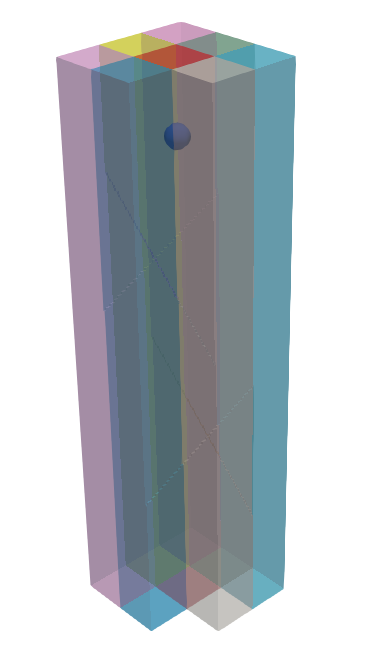
\includegraphics[width=7cm]{GWU_Thesis_Sarmakeeva/Images/chap3/decomp_9.png}
\subcaption{}
\label{fig:3figsA}}
\qquad
\begin{minipage}{7cm}
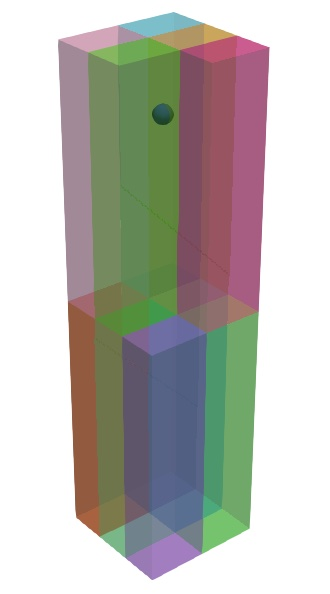
\includegraphics[width=7cm]{GWU_Thesis_Sarmakeeva/Images/chap3/decomp12.jpg}
\subcaption{}
\end{minipage}
\newline
\begin{minipage}{7cm}
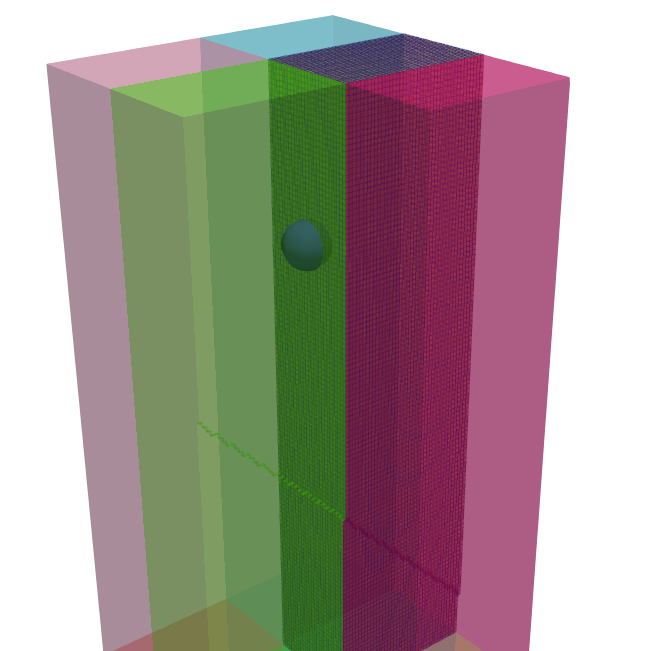
\includegraphics[width=5cm]{GWU_Thesis_Sarmakeeva/Images/chap3/decomp12_zoom.png}
\subcaption{}
\end{minipage}
\caption{Mesh decomposition a) 9 domains b) 12 domains c) zoomed mesh decomposition for 12 domains, where sphere intersected by 2 domains}
\label{decompositopn}
\end{figure}

It was situated precisely at the intersection of four domains. As shown on the Figure \ref{decompositopn}. This unfortunate placement was the root cause of the velocity spike. Once we addressed this issue by adjusting the mesh to avoid such intersections, the results stabilized and showed strong agreement with previously published data, confirming the reliability of our simulations. It would probably affect the movements of clumps, but because it will be a mixture of the bodies of different shapes, it would averaged on the domain.


%\subsection{Time step calculation}

%To run simulations with CFDEMcoupling we need to set up time step for DEM and for CFD solvers separately. It is common to use Courant (or Courant-Friedrichs-Lewy) number as a reference to get a solution converge. 

%To calculate time step we will use relationship:
%\begin{equation}
%   \Delta t =  \frac{CFL \times \Delta x}{\mathbf{u}},
%\end{equation}
%where $\mathbf{u}$ - fluid velocity, $\Delta t$ - time step, $\Delta x$ - grid size and $CFL \in \mathbb{Q}$ is the Courant number. It indicates the number of cells a \textit{fluid particle} passes in one time step. Consequently, a calculation can only be considered stable if the Courant number is smaller or equal to one.

\section{Multispherical bodies settings}

It took a while to set up multispherical bodies in the computational case. There are a lot of tutorials and material how to use OpenFoam solvers and how to create them, how to solve governing equations, however it is not the case for LIGGGHTS code. To clarify how to run example with multispherical bodies, we providing listing of the code with the main details.

\begin{lstlisting}[caption={LIGGGHTS Script}, label={lst:liggghts-script}]
#Multisphere

atom_style	sphere
atom_modify	map array sort 0 0
boundary	m m m
newton		off
communicate	single vel yes
processors	2 3 2
units		si
region		reg block 0.0 4.0 0.0 3.0 0. 4.0 units box
create_box	1 reg
neighbor	0.004 bin
neigh_modify	delay 0

#Material properties required for new pair styles
fix 		m1 all property/global youngsModulus peratomtype 1.e7
fix 		m2 all property/global poissonsRatio peratomtype 0.45
fix 		m3 all property/global coefficientRestitution peratomtypepair 1 0.3
fix 		m4 all property/global coefficientFriction peratomtypepair 1 0.5
fix 		m5 all property/global characteristicVelocity scalar 2.

#New pair style
pair_style gran model hertz tangential history #Hertzian without cohesion
pair_coeff	* *
timestep	0.00005
fix		gravi all gravity 9.81 vector 0.0 0.0 -1.0
fix zwalls all wall/gran model hertz tangential history primitive type 1 zplane 0.0
# cfd coupling
fix     cfd  all couple/cfd couple_every 10 mpi
fix     cfd2 all couple/cfd/force

#distributions for insertion
fix		pts1 all particletemplate/multisphere 15485863 atom_type 1 density constant 2500 nspheres 18 ntry 1000000 spheres file ../DEM/data/stone_small.multisphere scale 0.002 type 1
fix		pdd1 all particledistribution/discrete 1.  1 pts1 1.0
#region and insertion
region		bc block 0.2 0.4 0.0 0.2 0.0 0.3 units box
fix		ins all insert/pack seed 100001 distributiontemplate pdd1 vel constant 0. 0. -1. &
		insert_every once overlapcheck yes region bc ntry_mc 10000 volumefraction_region 0.4
#integrator for multisphere rigid bodies
fix		integr all multisphere
#output settings, include total thermal energy
compute		1 all erotate/sphere
fix		ts all check/timestep/gran 1000 0.1 0.1
thermo_style	custom step atoms ke c_1 f_ts[1] f_ts[2] vol
thermo		1000
thermo_modify	lost ignore norm no
compute_modify	thermo_temp dynamic yes
#insert the first particles so that dump is not empty
dump            dmp all custom 100 ../DEM/post/dump.data*.vtk id type x y z vx vy vz fx fy fz omegax omegay omegaz radius

#insert particles
run		1
\end{lstlisting}
First parameter which we need to adjust, after the number of processors for parallel execution in line 8, is in line 12 the  \texttt{region}
\begin{verbatim}
region		reg block 0.0 4.0 0.0 3.0 0.0 4.0 units box
\end{verbatim}
It is should have the same dimensions as CFD mesh. In the presented example for the region used block with dimensions $4 \times 3 \times 4$ for $x$, $y$, $z$ coordinates correspondingly. Could be set up as a different shapes, cone, prism or cylinder, more options in documentation LIGGGHTS. Then in line 12 :
\begin{verbatim}
neighbor	0.004 bin
\end{verbatim}
Neighbor lists store pairs of atoms that are potential interaction candidates. Each atom pair within a certain cutoff distance is included in this list. \texttt{bin} style is efficient and scales linearly with N/P. It's suitable for most cases and 0.004 is an additional length added to the interaction cutoff distance between particles. Line 33 
\begin{verbatim}
    fix		pts1 all particletemplate/multisphere 15485863 
    atom_type 1 density constant 2500 nspheres 18 ntry 1000000
    spheres file ../DEM/data/stone_small.multisphere scale 0.002 type 1
\end{verbatim}
responsible for multispherical body upload and insertion, where \verb|ntry| is the number of attempts made in the process of randomly positioning or orienting particles within the simulation space, utilizing a Monte Carlo technique. Another important parameter is \verb|scale| depends of that we can regulate the size of the clump and the amount of inserted particles correspondingly. 

Line 36 responsible for the area where multispherical bodies will be inserted. Same as computational area could be set up.
\begin{verbatim}
    region		bc block 0.2 0.4 0.0 0.2 0.0 0.3 units box
\end{verbatim}
Code in lines 37-38,
\begin{verbatim}
    fix		ins all insert/pack seed 100001 distributiontemplate pdd1
    vel constant 0. 0. -1. & insert_every once overlapcheck yes region 
    bc ntry_mc 10000 volumefraction_region 0.4
\end{verbatim}
keyword \texttt{volumefraction\_region}, is used to define a target volume fraction for the insertion of particles in a specified region. The volume fraction is a ratio that describes how much of the region's volume is occupied by particles. It's calculated as the total volume of inserted particles divided by the total volume of the region. This parameter modifies how many particles will be inserted in the particle region.

In the line 50 the command 
\begin{verbatim}
dump dmp all custom 100
\end{verbatim}
means how often output will be saved, where and the format data output.
We described the main important parameters which could be adjusted for different type of calculation. More details could be found in the documentation of the LIGGGHTS.


\subsection{Computational efficiency}
The algorithm presented on the Fig \ref{fig:cfddemSolver} is not straightforward. We need to pass back and forth data from one system to another. Thanks to API incorporated by a CFDEMcoupling developers team, there was no need to develop this part. API works as as follows: 
\begin{itemize}
    \item Set up equation which needed to be solved on fluid side.
    \item Create a force model with CFDEMcoupling, calculate how solid body affect fluid.
    \item Set up LIGGGHTS\textsuperscript{\textregistered} code, receive data form OpenFOAM\textsuperscript{\textregistered} through CFDEMcoupling force model, calculate the solid body motion.
\end{itemize}

The software combination takes a lot of resources, and API is done using MPI and all processes could be run parallel on the CPU. When we increase the domain size or number of particles, the number of CPU time required for running the simulation rises due to an increase in computational load.

The DEM calculations take ~1/8 of all computational time. The VOF part takes ~1/4, and parallel communication takes around the same resources as the DEM part. About half of the primary consumption comes from mapping the Lagrangian DEM data to an Eulerian field. This step is critical for the immersed boundary method because the velocity of the solid bodies is required to support a continuous forcing approach. Around the same computational resources as DEM calculations needed for parallel communication. This computational load shows that mapping procedure could be improved in the feature works.

\subsection{Conclusion}
In this chapter, we provided information on how the main algorithm works and provided information about the implementation of 3D parallel solver \verb|cfdemSolverInterFlowIB|. The force calculation is done with forceModel, which provides the interaction between fluid and particles, considering various physical phenomena like viscous and pressure drag and lift forces due to density differences. This information is then sent to the DEM module to update particle data, necessitating the inclusion of corresponding physics in the forceModel implementation.

Discussed features of how better to run mesh decomposition for basic test cases and how velocity could be affected due to the intersection of the body on the domain boundaries. We also provided an example of an input file for a multispherical body setup since it could be a challenging task. In the end, we discussed the computational efficiency of every part of the solver and that the majority of the computational resources comes from mapping the Lagrangian DEM data to an Eulerian field. In the next chapter we providing validation and verification of described in this chapter solver along with examples of simulation. 
